\begin{onehalfspace}
\section{Motivation}
\subsection{Problemstellung}
\label{s:intro}
Das übergeordnete Ziel für die Bausoftware ORCA AVA ist es, möglichst viele Informationen aus 3D-Modellen in der Ausschreibungssoftware automatisch importieren zu können. Das spart dem Architekten viel Zeit am Anfang in der Ausschreibung seines Projektes. Ein Teil, der aus den Modellen übernommen werden soll, sind Baustoffe und Materialien des Objektes. In der Arbeit geht es um die Übernahme dieser Baustoffe.
Als öffentliches Standardformat für 3D-Gebäudemodelle gibt es IFC, welches auch in der ORCA AVA benutzt wird. In diesen Modellen können auch die Materialien der einzelnen Bauteile spezifiziert werden. Diese können an verschiedenen Stellen an einem Bauteil im Modell angegeben werden. Für Materialbezeichnungen gibt es auch keine richtigen Standards. Hier besteht das Problem, dass das Textfeldern für die Materialangabe ein offenes Textfeld ist und somit kein Standard existiert und jedes IFC-Modell anders strukturiert ist. Deswegen ist das Ergebnis jeder Kostengliederung anders und vom jeweiligen Modell abhängig.

\subsection{Ziel}
Ziel ist es eine Kostengliederungsstruktur in der Bausoftware ORCA AVA aus den Materialeininformationen einer IFC-Datei zu generieren. Diese Kostengliederung kann am Anfang eines Projektes einmal importiert werden. Wenn dann im Laufe des Ausschreibungsprozesses ein Bauteil aus der IFC-Datei in die ORCA AVA übernommen wird, soll es automatisch einem Material in dieser Kostengliederungsstruktur zugewiesen werden. So kann man das ausgeschriebene Gebäude nach den Materialangaben auswerten.
\\


Ein Algorithmus soll zuerst die Möglichkeiten der Materialangabe in der IFC-Datei zusammenführen. Mit Hilfe von Natural Language Processing und Artificial Inteligence eine Lösung entwickelt werden, um eine klassifizierte und standardisierte Liste der Materialien zu erschaffen. 


\section{Forschungsstand}
\section{Vorläufige Gliederung}
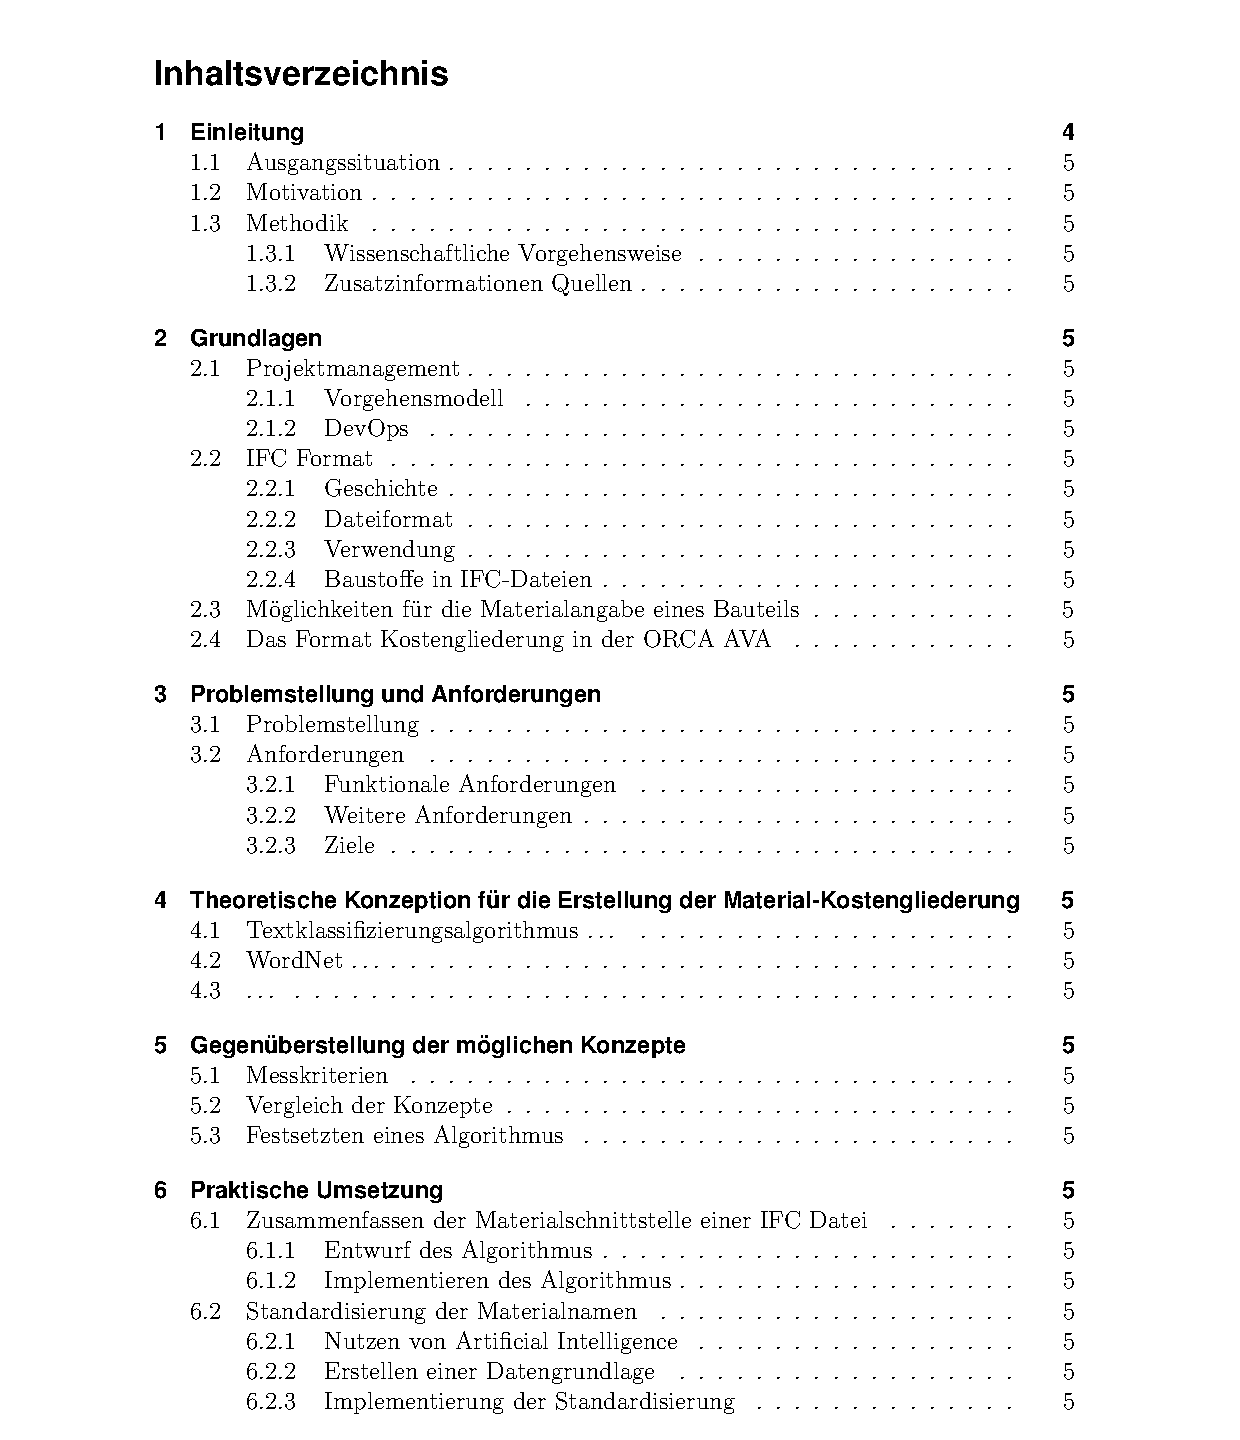
\includepdf[pages=-]{figures/inhaltsverzeichnis.pdf}
\section{Zeitplan}

\begin{description}
	\item[1.]
	Recherchieren über verschiedene mögliche Techniken und Algorithmen
	\item[2.] 
	Austesten der gefundenen Algorithmen
	\item[3.]
	Messen der Ergebnisse der Algorithmen
	\item[4.] Implementieren des besten Ergebnisses
\end{description}

\section{Erste Literatur}
\end{onehalfspace}